\documentclass{article}
\usepackage{graphicx}
\usepackage{amsmath}
\usepackage{enumitem}
\usepackage[margin=1in]{geometry}
\usepackage{float}
\usepackage{tikz}
\usetikzlibrary{positioning}

\begin{document}

\begin{center}
{\Large \textbf{Machine Learning Supervised Learning Quiz - Set 1}}
\end{center}

\vspace{0.5cm}

\textbf{Instructions:}
\begin{itemize}
\item Answer all questions clearly and completely.
\item Show your work for subjective questions.
\item For multiple choice questions, circle the correct option.
\item \textbf{Total marks: 79} (MCQ: 21 marks, Subjective: 58 marks)
\end{itemize}

\vspace{0.5cm}


\section*{Multiple Choice Questions}

\textbf{Q1.} Which regularization technique adds a penalty term proportional to the sum of absolute values of parameters? \textbf{[2 marks]}

\begin{enumerate}[label=(\Alph*)]

  \item L1 Regularization (Lasso)

  \item Dropout

  \item Elastic Net

  \item L2 Regularization (Ridge)

\end{enumerate}

\vspace{0.3cm}

\textbf{Q2.} In Support Vector Machines, what happens when the regularization parameter C is very large? \textbf{[3 marks]}

\begin{enumerate}[label=(\Alph*)]

  \item The model focuses on minimizing training error and may overfit

  \item The kernel function becomes linear

  \item The model becomes more regularized and may underfit

  \item The support vectors are ignored

\end{enumerate}

\vspace{0.3cm}

\textbf{Q3.} Looking at the ROC curve below:

\begin{center}
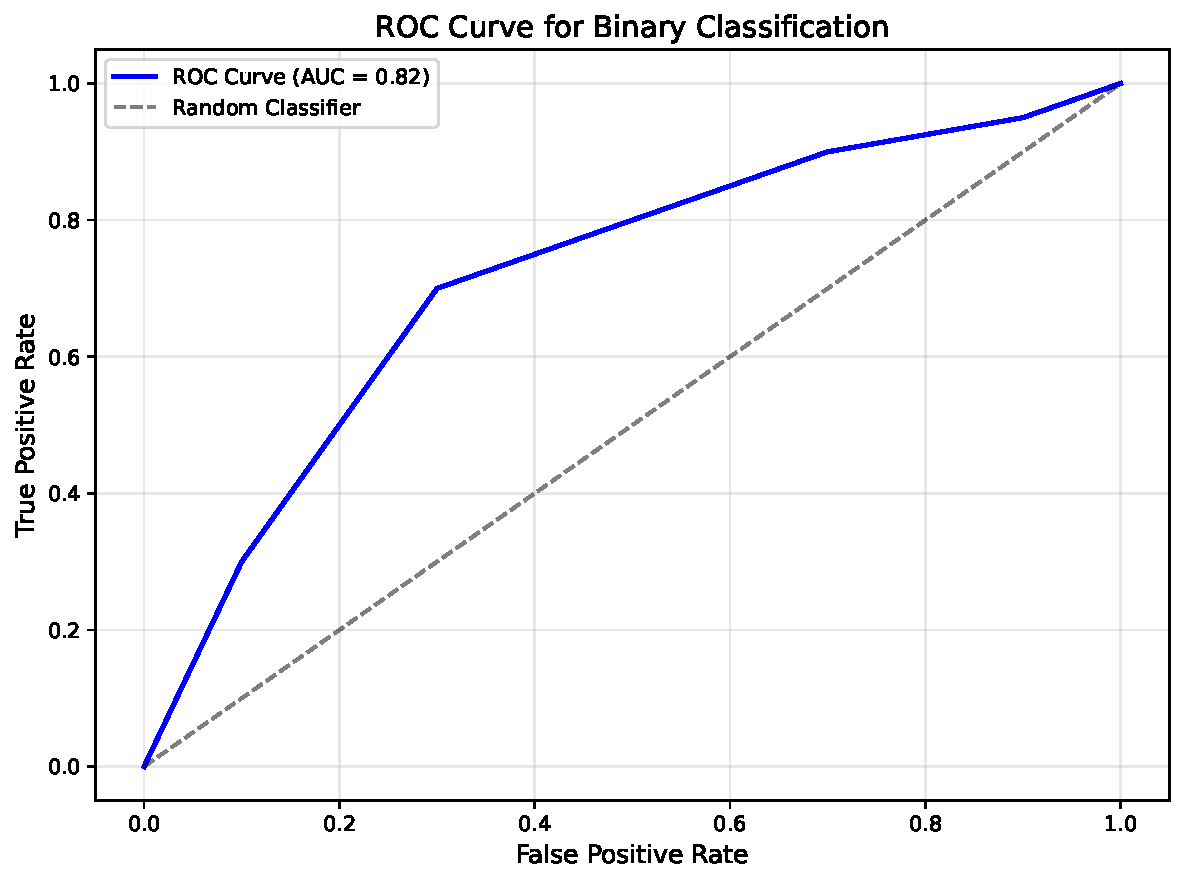
\includegraphics[width=0.6\textwidth]{figures/roc_curve.pdf}
\end{center}

What does the area under the curve (AUC) represent? \textbf{[3 marks]}

\begin{enumerate}[label=(\Alph*)]

  \item The total number of correct predictions

  \item The difference between true positive rate and false positive rate

  \item The computational complexity of the algorithm

  \item The probability that the classifier ranks a random positive instance higher than a random negative instance

\end{enumerate}

\vspace{0.3cm}

\textbf{Q4.} In the neural network architecture shown:

\begin{center}

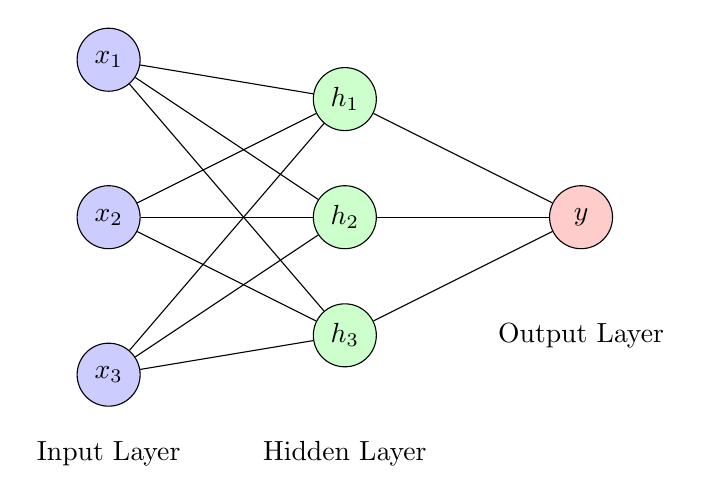
\begin{tikzpicture}[
  node distance=2cm,
  neuron/.style={circle, draw, minimum size=0.8cm},
  input/.style={neuron, fill=blue!20},
  hidden/.style={neuron, fill=green!20},
  output/.style={neuron, fill=red!20}
]

% Input layer
\node[input] (i1) at (0,2) {$x_1$};
\node[input] (i2) at (0,0) {$x_2$};
\node[input] (i3) at (0,-2) {$x_3$};

% Hidden layer
\node[hidden] (h1) at (3,1.5) {$h_1$};
\node[hidden] (h2) at (3,0) {$h_2$};
\node[hidden] (h3) at (3,-1.5) {$h_3$};

% Output layer
\node[output] (o1) at (6,0) {$y$};

% Connections
\foreach \i in {1,2,3}
  \foreach \h in {1,2,3}
    \draw (i\i) -- (h\h);

\foreach \h in {1,2,3}
  \draw (h\h) -- (o1);

% Labels
\node at (0,-3) {Input Layer};
\node at (3,-3) {Hidden Layer};
\node at (6,-1.5) {Output Layer};

\end{tikzpicture}

\end{center}

How many parameters (weights and biases) does this network have? \textbf{[4 marks]}

\begin{enumerate}[label=(\Alph*)]

  \item 13

  \item 16

  \item 15

  \item 12

\end{enumerate}

\vspace{0.3cm}

\textbf{Q5.} In a decision tree, which impurity measure is most commonly used for classification tasks? \textbf{[2 marks]}

\begin{enumerate}[label=(\Alph*)]

  \item Mean Absolute Error (MAE)

  \item Gini Impurity

  \item Mean Squared Error (MSE)

  \item R-squared

\end{enumerate}

\vspace{0.3cm}

\textbf{Q6.} Which of the following is true about k-fold cross-validation? \textbf{[2 marks]}

\begin{enumerate}[label=(\Alph*)]

  \item It splits data into k parts, trains on k-1 parts, tests on 1 part, repeats k times

  \item It requires k different algorithms

  \item It uses k different datasets for training

  \item It only works when k equals the number of features

\end{enumerate}

\vspace{0.3cm}

\textbf{Q7.} Which of the following best describes the bias-variance tradeoff in machine learning? \textbf{[2 marks]}

\begin{enumerate}[label=(\Alph*)]

  \item High bias models always perform better than high variance models

  \item Reducing bias typically increases variance, and vice versa

  \item Bias and variance are independent and don't affect each other

  \item Variance only matters in unsupervised learning

\end{enumerate}

\vspace{0.3cm}

\textbf{Q8.} Given the confusion matrix below for a binary classification problem:

\begin{center}
\begin{tabular}{|c|c|c|}
\hline
 & \textbf{Predicted 0} & \textbf{Predicted 1} \\
\hline
\textbf{Actual 0} & 85 & 15 \\
\hline
\textbf{Actual 1} & 10 & 90 \\
\hline
\end{tabular}
\end{center}

What is the precision of the classifier? \textbf{[3 marks]}

\begin{enumerate}[label=(\Alph*)]

  \item 0.90

  \item 0.875

  \item 0.85

  \item 0.857

\end{enumerate}

\vspace{0.3cm}




\section*{Subjective Questions}

\textbf{Q9.} \textbf{[Total: 7 marks]} Examine the overfitting comparison plots:

\begin{center}
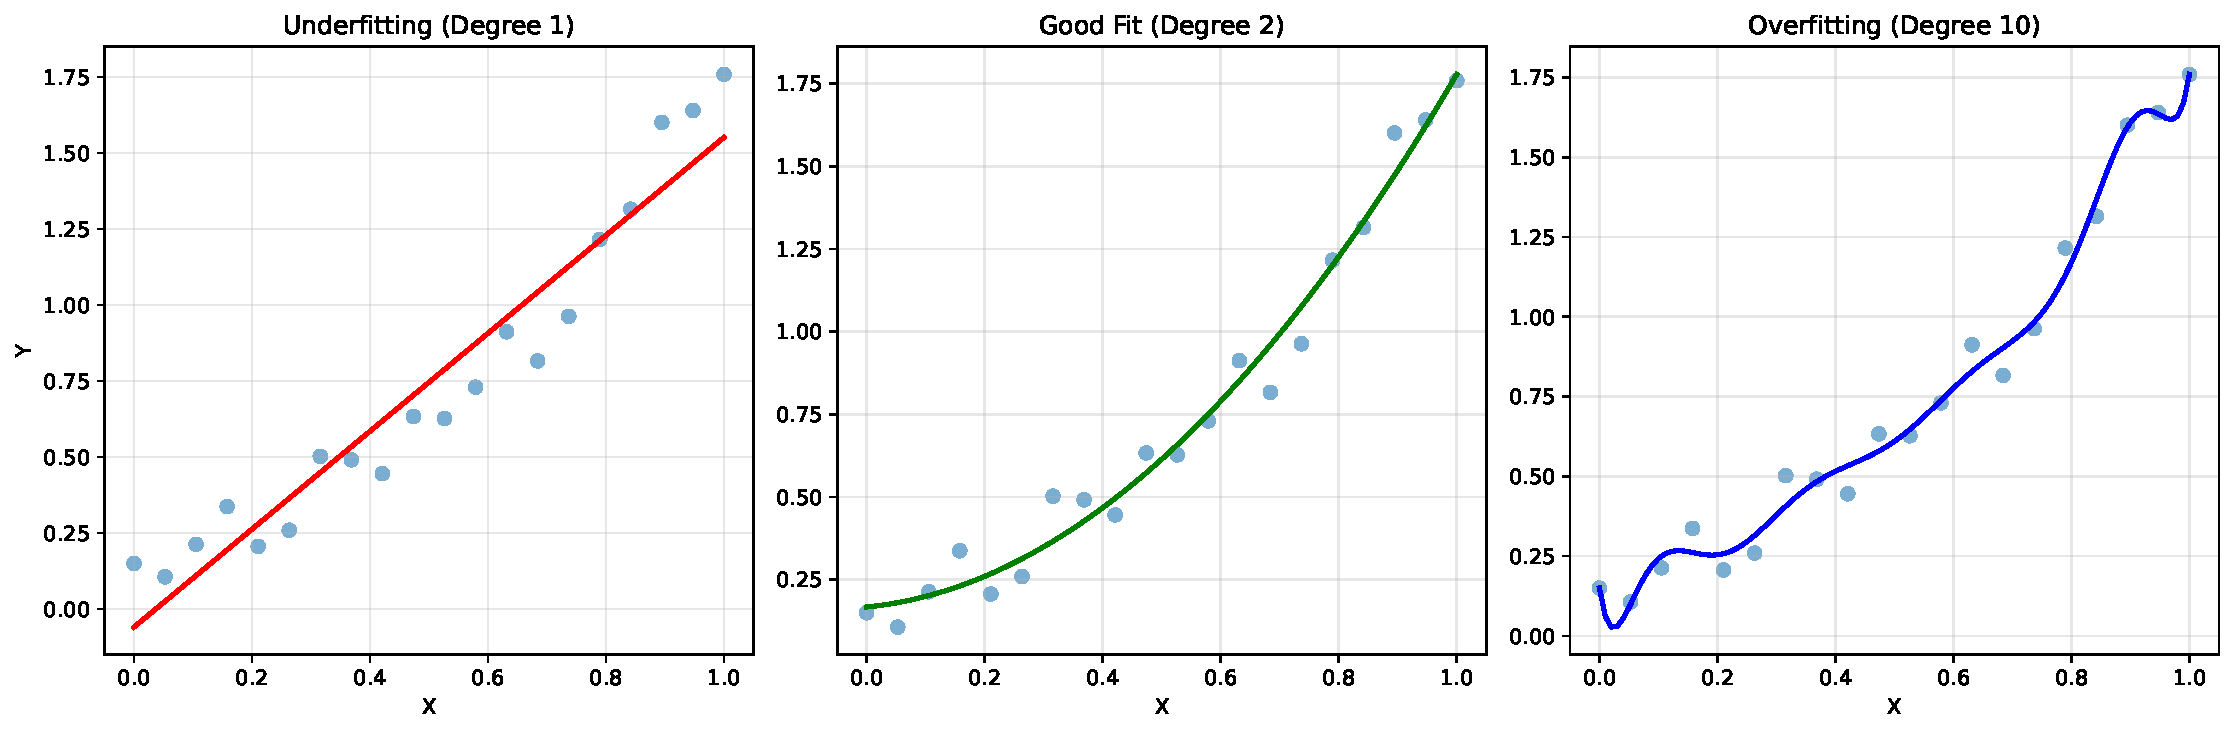
\includegraphics[width=0.9\textwidth]{figures/overfitting_comparison.pdf}
\end{center}

\textbf{a)} Identify which model suffers from underfitting, good fit, and overfitting. Justify each choice. \textbf{[4 marks]}

\textbf{b)} If you had to choose a regularization parameter $\lambda$ for ridge regression, would you choose a high or low value to move from the overfitted model to the good fit model? Explain. \textbf{[3 marks]}


\textbf{Q10.} \textbf{[Total: 9 marks]} Compare and contrast the following three supervised learning algorithms in terms of their assumptions, strengths, and weaknesses:

\begin{center}
\begin{tabular}{|p{3cm}|p{3cm}|p{3cm}|p{3cm}|}
\hline
\textbf{Algorithm} & \textbf{Key Assumptions} & \textbf{Strengths} & \textbf{Weaknesses} \\
\hline
Linear Regression & & & \\
\hline
Decision Trees & & & \\
\hline
k-NN & & & \\
\hline
\end{tabular}
\end{center}

Fill in the table above and provide a brief explanation for each entry. \textbf{[9 marks]}


\textbf{Q11.} \textbf{[Total: 10 marks]} Explain the ensemble methods Random Forest and AdaBoost:

\textbf{a)} Describe how Random Forest reduces overfitting compared to a single decision tree. \textbf{[3 marks]}

\textbf{b)} Explain the boosting principle in AdaBoost and how it differs from bagging. \textbf{[4 marks]}

\textbf{c)} Under what circumstances would you prefer Random Forest over AdaBoost and vice versa? \textbf{[3 marks]}


\textbf{Q12.} \textbf{[Total: 6 marks]} Given the learning curves shown below:

\begin{center}
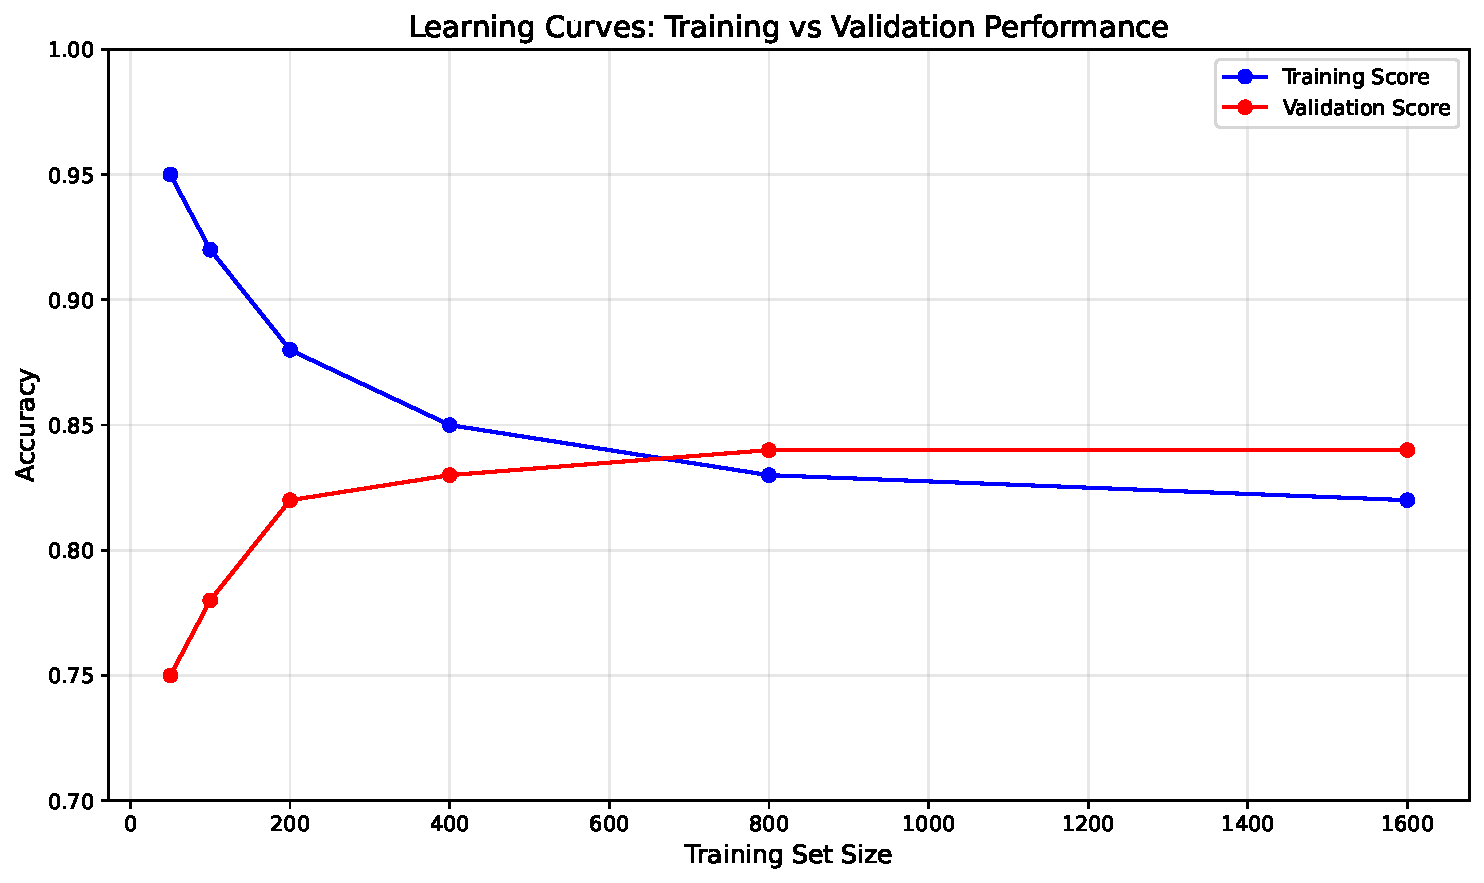
\includegraphics[width=0.8\textwidth]{figures/learning_curves.pdf}
\end{center}

\textbf{a)} Identify whether the model is suffering from high bias or high variance. Justify your answer. \textbf{[3 marks]}

\textbf{b)} Suggest two specific techniques to improve the model performance. \textbf{[2 marks]}

\textbf{c)} If the training accuracy is 82\% and validation accuracy is 79\%, calculate the overfitting gap. \textbf{[1 mark]}


\textbf{Q13.} \textbf{[Total: 8 marks]} Derive the gradient descent update rule for logistic regression. Start from the logistic loss function:

$$J(\theta) = -\frac{1}{m} \sum_{i=1}^{m} [y^{(i)} \log(h_\theta(x^{(i)})) + (1-y^{(i)}) \log(1-h_\theta(x^{(i)}))]$$

where $h_\theta(x) = \frac{1}{1 + e^{-\theta^T x}}$

Show all steps clearly including the partial derivatives. \textbf{[8 marks]}


\textbf{Q14.} \textbf{[Total: 7 marks]} Consider the SVM with margin illustration:

\begin{center}

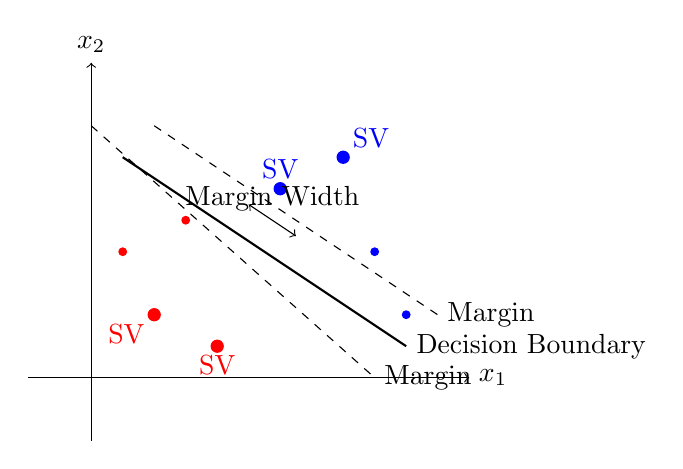
\begin{tikzpicture}[scale=0.8]
% Draw axes
\draw[->] (-1,0) -- (6,0) node[right] {$x_1$};
\draw[->] (0,-1) -- (0,5) node[above] {$x_2$};

% Draw support vectors
\fill[red] (1,1) circle (3pt) node[below left] {SV};
\fill[red] (2,0.5) circle (3pt) node[below] {SV};
\fill[blue] (3,3) circle (3pt) node[above] {SV};
\fill[blue] (4,3.5) circle (3pt) node[above right] {SV};

% Draw other points
\fill[red] (0.5,2) circle (2pt);
\fill[red] (1.5,2.5) circle (2pt);
\fill[blue] (4.5,2) circle (2pt);
\fill[blue] (5,1) circle (2pt);

% Draw decision boundary and margins
\draw[thick] (0.5,3.5) -- (5,0.5) node[right] {Decision Boundary};
\draw[dashed] (0,4) -- (4.5,0) node[right] {Margin};
\draw[dashed] (1,4) -- (5.5,1) node[right] {Margin};

% Add margin width indicator
\draw[<->] (2.5,2.75) -- (3.25,2.25) node[midway,above] {Margin Width};

\end{tikzpicture}

\end{center}

\textbf{a)} Explain the concept of support vectors and their role in SVM. \textbf{[3 marks]}

\textbf{b)} If we have 120 positive samples and 80 negative samples, and 15 of them are support vectors, what percentage of the data points are support vectors? \textbf{[2 marks]}

\textbf{c)} Compare the computational complexity of SVM prediction with and without kernel tricks. \textbf{[2 marks]}


\textbf{Q15.} \textbf{[Total: 5 marks]} Consider the following dataset for linear regression:

\begin{center}
\begin{tabular}{|c|c|c|c|}
\hline
\textbf{Sample} & \textbf{Feature 1} & \textbf{Feature 2} & \textbf{Target} \\
\hline
1 & 1 & 2 & 6 \\
\hline
2 & 3 & 1 & 7 \\
\hline
3 & 2 & 3 & 9 \\
\hline
4 & 4 & 2 & 10 \\
\hline
\end{tabular}
\end{center}

\textbf{a)} Calculate the mean squared error (MSE) if the model predicts $\hat{y} = 5.9, 7.1, 8.8, 9.9$ respectively. \textbf{[3 marks]}

\textbf{b)} If we use L2 regularization with $\lambda = 0.05$, write the complete loss function. \textbf{[2 marks]}


\textbf{Q16.} \textbf{[Total: 6 marks]} Analyze the decision tree structure below:

\begin{center}

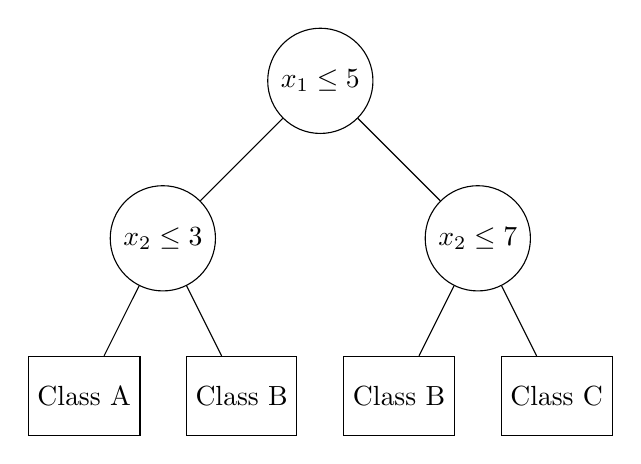
\begin{tikzpicture}[
  level distance=2cm,
  level 1/.style={sibling distance=4cm},
  level 2/.style={sibling distance=2cm},
  every node/.style={circle, draw, minimum size=1cm}
]
\node {$x_1 \leq 5$}
  child { node {$x_2 \leq 3$}
    child { node[rectangle] {Class A} }
    child { node[rectangle] {Class B} }
  }
  child { node {$x_2 \leq 7$}
    child { node[rectangle] {Class B} }
    child { node[rectangle] {Class C} }
  };
\end{tikzpicture}

\end{center}

\textbf{a)} What is the maximum depth of this tree? \textbf{[1 mark]}

\textbf{b)} Calculate the Gini impurity for a node with class distribution: Class A: 40 samples, Class B: 30 samples, Class C: 10 samples. \textbf{[3 marks]}

\textbf{c)} Explain why pruning might be beneficial for this tree. \textbf{[2 marks]}




\end{document}